\section{Introduction}
\label{sec-intro}


Visual Question Answering (\vqa), the
problem of automatically and efficiently answering questions about visual content, has attracted a wide range of attention, since it has a variety of applications in \eg image captioning, surveillance video understanding, visual commentator robot, \etc. 
Though important, the \vqa problem brings a rich set of challenges spanning various domains such as computer vision, natural language processing, knowledge representation, and reasoning. 
In recent years, \vqa has achieved significant
progress, owing to the development of deep architectures suited for this task and the creation of large \vqa datasets to train these models. 
However, a number of studies~\cite{peixi2019,Goyal_2017} also pointed out that despite recent progress, today's neural network based approaches demonstrate a few weaknesses, which greatly hinders its further development. First of all, existing techniques train deep neural networks to predict answers, where image-question pairs are jointly embedded as training data, following this way, the correlation between the question and the image is ignored, which may lead to difficulty in balancing accuracy and efficiency. Secondly, deep neural networks works as ``black boxes'', it is very hard to identify the causal relations between network design and system performance, not to mention ensuring acceptable performance. Lastly, due to lack of reasoning capability, a host of existing techniques show poor performance when answering real-life questions, that are often open-ended and require necessary reasoning. Though a novel method~\cite{peixi2019} with reasoning capability is proposed, the method shows difficulty in generalization.  

To address the issues mentioned above, a method, that finds answers based on the understanding of the questions and necessary reasoning, is required. 


\begin{figure}[tb]
\centering
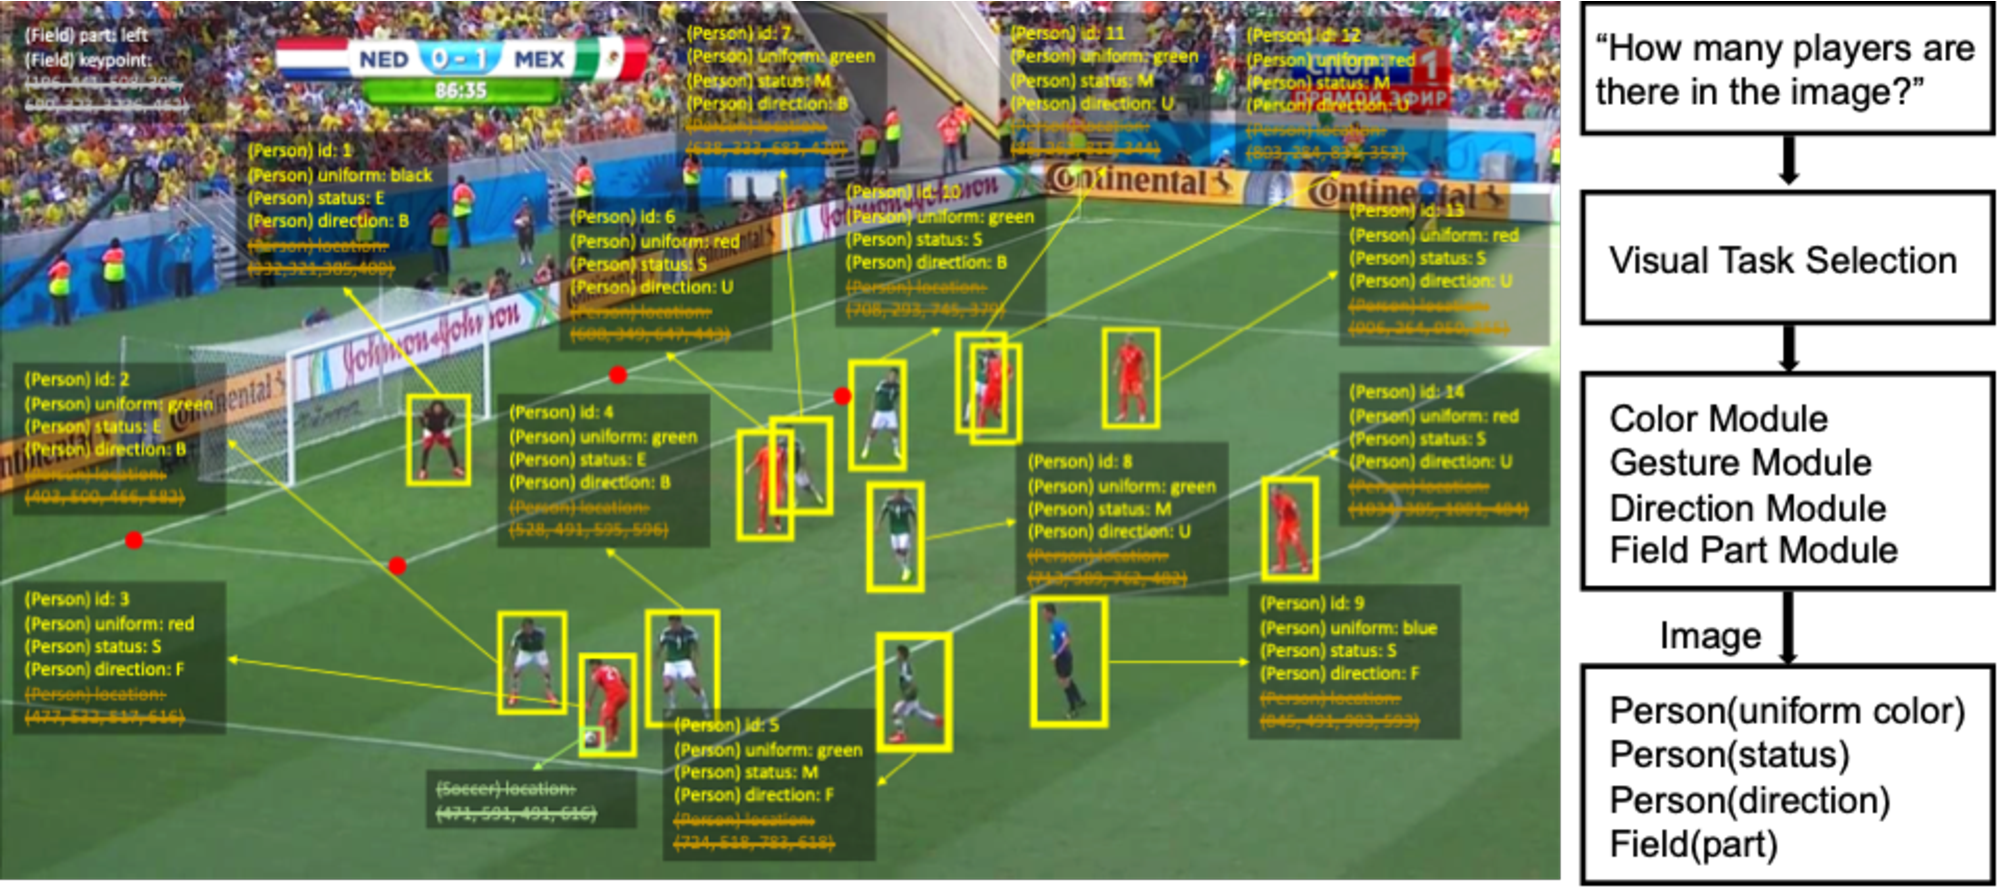
\includegraphics[width=\columnwidth]{figures/motivation.eps}
\caption{The image is about soccer match, where each person object is associated with attributes: id, uniform color, status (\underline{S}tanding, \underline{M}oving, \underline{E}xpansion), direction (\underline{B}acking, \underline{F}acing, \underline{N/A}), as well as location, and the soccer object is attributed with location. However, not all informations are necessary in answering one question, visual tasks are selected to achieve acquiring relevant information.%Part (b) shows a part of corresponding entity-attribute graph. Part (c) exhibits a $\nlq$ and its corresponding query graph $Q$. 
}
\vspace{-4ex}
\label{fig:example}
\end{figure}


\begin{example}
\Cref{fig:example} depicts an image about a soccer match, where each object is associated with a set of attributes. A typical question may ask ``How many players are there in the image?''. Though simple, it is a challenging task to efficiently answer the query, since (1) traditionally, it often takes time to extract as much information as possible from the given image, and then answer the questions; while, only question related objects are needed; (2) information extracted from image alone is often insufficient to answer questions, hence missing values that are crucial for question answering should be inferred by certain reasoning techniques. \looseness=-1

To tackle the issues, one may (1) model input \ie image and question, with graph structures that can capture information from both image and question well, and ease question understanding and reasoning; (2) follow the work-flow given on the right hand side of \cref{fig:example} to identify correct graph representation of the question, and a set of policies that are closely related to the question and used to guide forthcoming visual tasks; and (3) infer values \eg ``role'' of person objects (referee, goalkeeper or player) using well trained classification model.  
\end{example}

This example suggests that we address the \vqa problem by modeling inputs as graphs, leveraging techniques to guide question translation, visual processing, and do reasoning. While to do this, two critical questions have to be answered. (1) How to understand questions and carry out question related visual tasks? (2) How to infer crucial information to assist question answering?  


\vspace{2ex}
\stitle{Contributions.} In contrast to a majority of deep neural networks based \vqa techniques, which not only overlooks correlation between questions and images, but also lacks of necessary reasoning, we provide a novel approach that integrates question understanding and reasoning, for the \vqa problem. The main contributions of the paper are as follow.  

(1) We model images and questions as graphs, and propose to answer visual questions with graph matching. This new representation and answering scheme constitute the base of our techniques.  

(2) We introduce a method to guide question translation and visual processing based on reinforcement learning. That is, given a question, our method can identify its correct graph representation, and a set of policies to guide visual tasks in a more efficient manner. 

(3) We provide a method to infer missing values to answer questions. The reasoning task relies on a classifier, that is generated by offline training with supervised learning. 

4) We conduct extensive experimental studies to verify the performance of our method on both our curated \vqa dataset and a public \vqa dataset. We find that our method outperforms statt-of-the-art methods on both datasets.